\phantomsection
%\addcontentsline{toc}{chapter}{Introduzione}
\chapter{Introduzione}
\markboth{Introduzione}{}
% [titolo ridotto se non ci dovesse stare] {titolo completo}
Il presente documento ha l'obiettivo di illustrare le metodologie utilizzate nell'ambito dell'attività progettuale svolta nel contesto del corso di \emph{Penetration Testing and Ethical Hacking}, tenuto dal prof. Arcangelo Castiglione presso l'Università degli studi di Salerno durante l'anno accademico 2022/2023. L'attività progettuale in questione consiste nello svolgimento del processo di \emph{Penetration Testing} su un asset vulnerabile \emph{by-design}; nello specifico, è stata scelta la macchina virtuale \emph{Momentum: 1} messa a disposizione sulla piattaforma \emph{VulnHub} dall'utente \emph{AL1ENUM}. 

\section{Processo di \emph{Penetration Testing}}
Il processo di \emph{Penetration Testing} è stato svolto in maniera conforme alle modalità illustrate durante il corso, pertanto sono state previste (in ordine) le seguenti fasi:
\begin{enumerate}
    \item \textbf{Target Scoping}: definizione degli accordi tra le parti coinvolte nel processo di \emph{Penetration Testing};
    \item \textbf{Information Gathering}: raccolta di informazioni relative all'asset sia dal punto di vista della parte umana che dal punto di vista tecnologico;
    \item \textbf{Target Discovery}: individuazione della macchina target all'interno della rete;
    \item \textbf{Target Enumeration}: enumerazione dei servizi erogati dalla macchina target;
    \item \textbf{Vulnerability Mapping}: individuazione delle vulnerabilità presenti sulla macchina target;
    \item \textbf{Target Exploitation}: sfruttamento delle vulnerabilità individuate nel corso della fase precedente, finalizzato all'ottenimento dell'accesso alla macchina target;
    \item \textbf{Privilege Escalation}: ottenimento dei massimi privilegi sulla macchina target al fine di acquisire ulteriori informazioni;
    \item \textbf{Maintaining Access}: realizzazione di opportuni software, chiamati \emph{backdoor}, volti al mantenimento dell'accesso sulla macchina target, in modo tale da evitare di dover rieseguire le precedenti fasi per accedervi nuovamente.
\end{enumerate}

\section{Strumenti utilizzati} 
Al fine di svolgere l'attività di \emph{Penetration Testing} è risultato necessario l'impiego di un ambiente di virtualizzazione che coinvolgesse la macchina target ed un'eventuale macchina attaccante dotata di opportuni strumenti utili all'analisi dell'asset vulnerabile. L'ambiente di virtualizzazione utilizzato è \emph{VirtualBox 7.0.8 r156879} mediante il quale è stata configurata una rete virtuale la cui infrastruttura verrà trattata nell'ambito del paragrafo successivo. La scelta del sistema operativo della macchina attaccante è ricaduta su \emph{Kali Linux} (di cui è stata installata la release \emph{2023.2}) in quanto risulta essere una delle distribuzioni \emph{Linux} più utilizzate nell'ambito di contesti come \emph{Cybersecurity, Penetration Testing} e \emph{Digital Forensics}. \emph{Kali Linux} fornisce diversi strumenti preinstallati, utili per l'analisi da svolgere; alcuni di questi strumenti sono stati ampiamente utilizzati nell'ambito del processo di \emph{Penetration Testing}, per cui verranno elencati e descritti nell'ambito della trattazione delle diverse fasi del processo svolto. 
\section{Infrastruttura di rete} 
La configurazione dell'infrastruttura di rete risulta cruciale in quanto permette la comunicazione tra la macchina target e quella attaccante, oltre a consentire a quest'ultima di collegarsi alla rete per aggiornare i tool di cui dispone ed accedere ai database di vulnerabilità, \emph{exploit} e \emph{payload}. Mediante l'apposito strumento messo a disposizione da \emph{VirtualBox} è stata realizzata una rete virtuale con \emph{NAT} avente come indirizzo \emph{IPv4 10.0.2.0/24}, alla quale sono state collegate le macchine virtuali \emph{Kali} e \emph{Momentum}. L'infrastruttura di rete è illlustrata nella figura \ref{fig:virtualbox} in una versione semplificata che non tiene conto degli host virtuali di \emph{VirtualBox} utilizzati per la gestione del \emph{NAT} e del \emph{DHCP}. 
\begin{figure}[h]
    \centering
    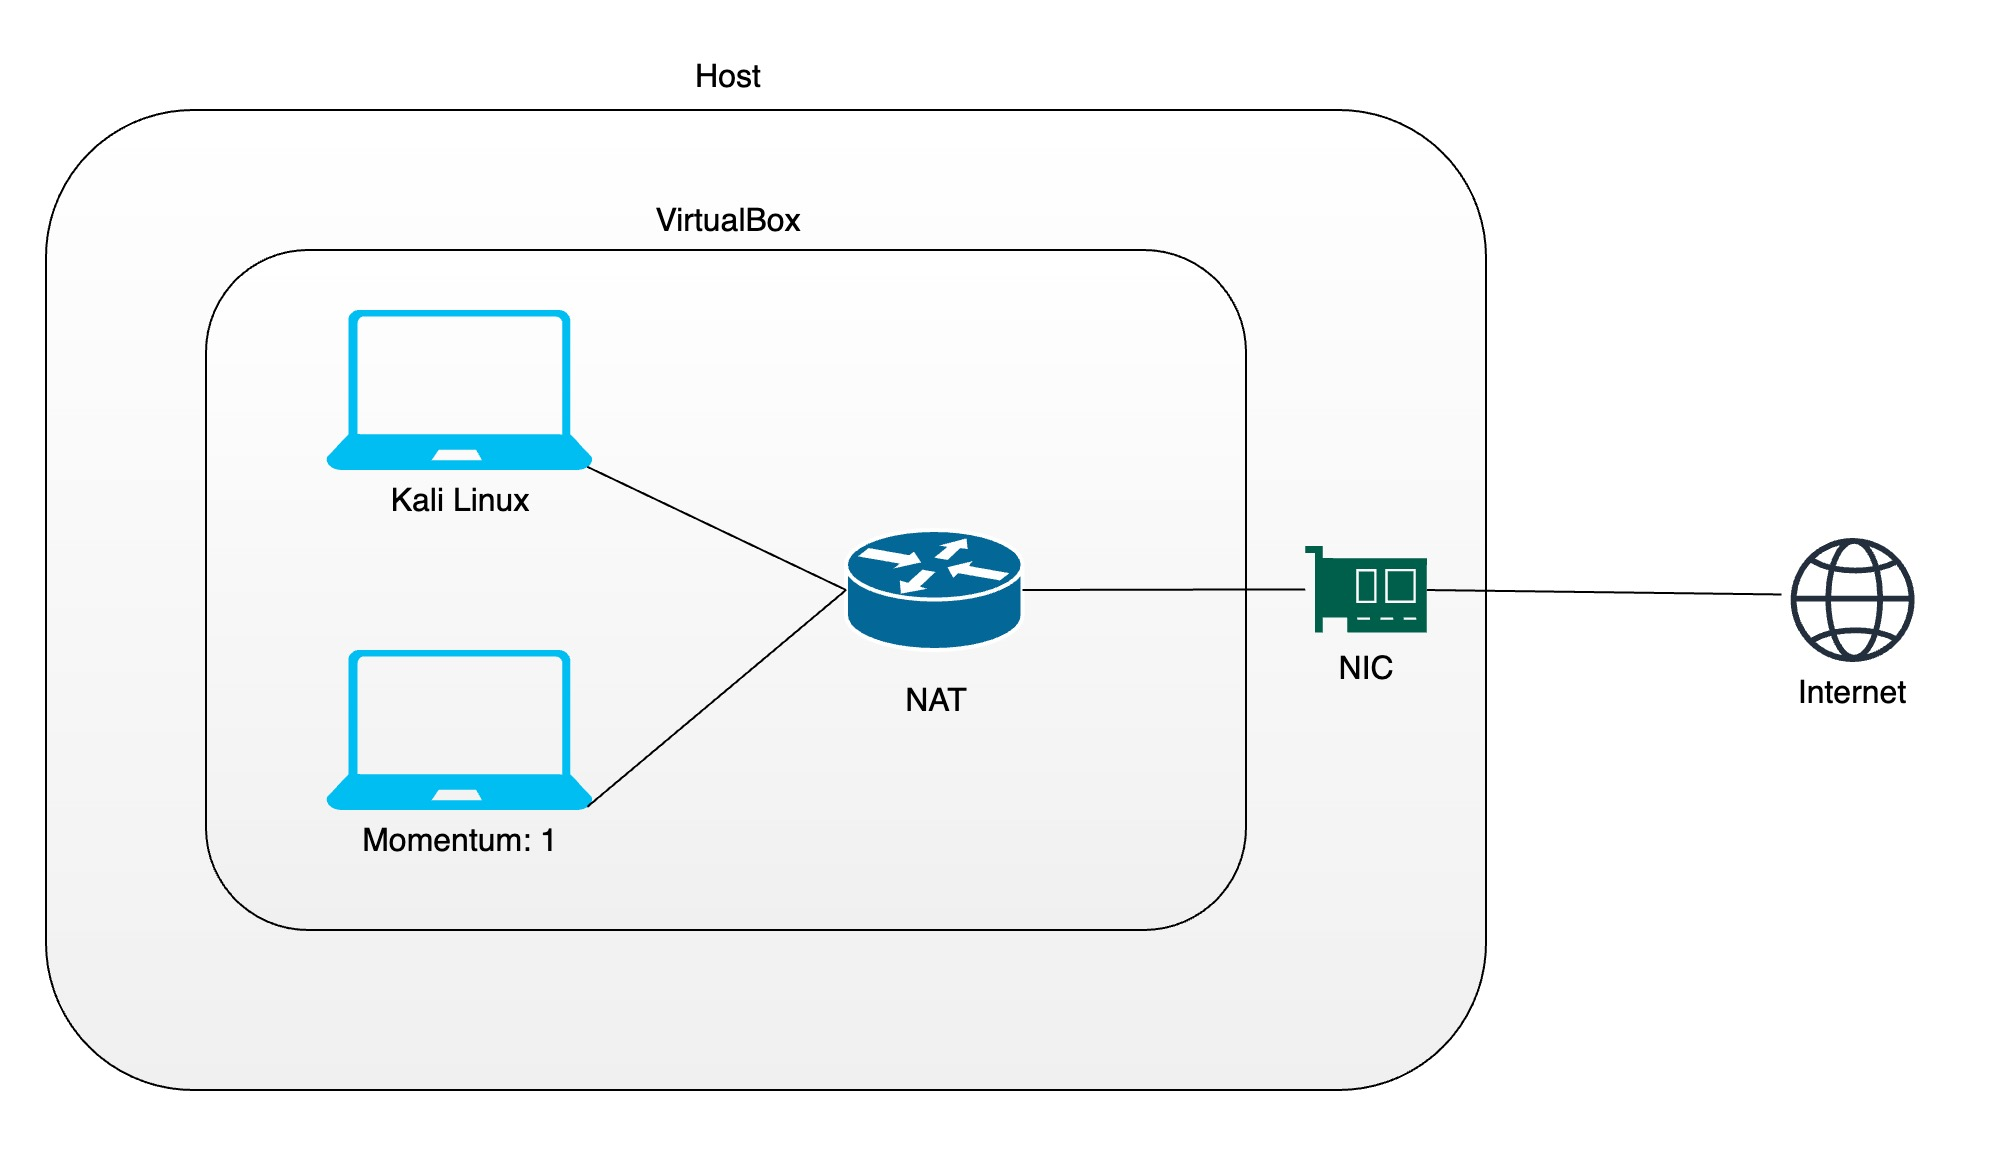
\includegraphics[scale=0.2]{capitoli/images/virtualbox.jpeg}
    \caption{Infrastruttura di rete virtuale}
    \label{fig:virtualbox}
\end{figure}
\section{Struttura del documento}
La presente trattazione verrà suddivisa in quattro capitoli:
\begin{itemize}
    \item Il primo capitolo fornisce una panoramica sulle fasi del lavoro svolto, sugli strumenti utilizzati e sull'infrastruttura della rete virtuale;
    \item Il secondo capitolo tratta la fase di \emph{Pre-Exploitation} che copre le fasi di \emph{Target Scoping, Information Gathering, Target Discovery} e \emph{Vulnerability Mapping};
    \item Il terzo capitolo tratta la fase di \emph{Target Exploitation};
    \item Il quarto capitolo tratta la fase di \emph{Post-Exploitation} che copre le fasi di \emph{Privilege Escalation} e \emph{Maintaining Access}.
\end{itemize}